% !TeX program = xelatex
% !TeX encoding = UTF-8
% --- 使用 ctexart 文档类，自动处理中文支持和排版 ---
\documentclass[a4paper]{ctexart}

% --- 导入宏包 ---
\usepackage{geometry} % 用于设置页边距
\usepackage{graphicx} % 用于插入图片
\usepackage{listings} % 用于排版代码
\usepackage{xcolor}   % 用于代码高亮颜色
\usepackage{enumitem} % 用于高级列表控制
\usepackage{hyperref} % 用于生成可点击的链接 (必须放在最后)

% --- 页面设置 ---
\geometry{a4paper, top=2.5cm, bottom=2.5cm, left=2.5cm, right=2.5cm}

% --- 代码高亮 (listings) 样式定义 (MATLAB) ---
\definecolor{codegray}{rgb}{0.5,0.5,0.5}
\definecolor{codepurple}{rgb}{0.58,0,0.82}
\definecolor{codegreen}{rgb}{0,0.5,0}

\lstdefinestyle{matlabstyle}{
	language=Matlab,
	basicstyle=\ttfamily\small,       % 代码字体
	commentstyle=\color{codegreen},     % 注释颜色
	keywordstyle=\color{blue},          % 关键词颜色
	stringstyle=\color{codepurple},     % 字符串颜色
	numberstyle=\tiny\color{codegray}, % 行号颜色
	breaklines=true,                  % 自动换行
	showstringspaces=false,
	frame=tb,                         % 上下边框
	captionpos=b,                     % 标题在底部
	numbers=left,                     % 行号在左侧
	numbersep=5pt,                    % 行号间距
	backgroundcolor=\color{gray!10}   % 浅灰色背景
}
\lstset{style=matlabstyle} % 全局应用此样式

% --- PDF 书签和链接设置 ---
\hypersetup{
	colorlinks=true,
	linkcolor=blue,
	urlcolor=blue,
	citecolor=blue,
	pdftitle={傅立叶分析和小波分析实验报告},
	pdfauthor={林鑫}
}

% --- 封面信息 ---
\title{傅立叶分析和小波分析实验报告}
\author{
	课程名称：傅立叶分析和小波分析 \\
	实验项目名称：基于小波变换的图像压缩 \\
	实验时间：2025.11.13 \\
	班级：信计2302班 \quad 姓名：林鑫 \quad 学号：1043220122
}
\date{} % 不显示默认日期

% --- 文档开始 ---
\begin{document}
	
	\maketitle      % 生成封面
	\tableofcontents % 生成目录
	\newpage
	
	\section{实验目的}
	\begin{enumerate}
		\item 理解小波变换（Wavelet Transform）的基本原理及其在图像处理中的应用。
		\item 掌握使用 MATLAB 对图像进行二维离散小波变换（2D-DWT）的分解与重构方法。
		\item 探究小波变换的能量集中特性，并基于此实现一个基本的图像压缩演示。
		\item 分析不同分解层次对图像压缩效果的影响。
	\end{enumerate}
	
	\section{实验原理与概念介绍}
	\subsection{图像压缩的基本概念}
	图像压缩是指减少表示一幅数字图像所需数据量的技术。其目的是在不（或在可接受范围内）降低图像质量的前提下，去除数据冗余，以便于图像的存储和传输。
	
	图像压缩分为两类：
	\begin{itemize}
		\item \textbf{无损压缩（Lossless Compression）：} 压缩和解压缩后的图像与原始图像完全一致，不丢失任何信息。
		\item \textbf{有损压缩（Lossy Compression）：} 压缩过程中会丢失一部分信息，解压缩后的图像与原始图像有差异，但人眼通常难以察觉。有损压缩通常能获得比无损压缩高得多的压缩比。
	\end{itemize}
	本实验所探究的小波压缩是一种典型的有损压缩技术，其基本流程包括三个步骤：\textbf{变换、量化和编码}。
	
	\subsection{小波变换（Wavelet Transform）}
	\subsubsection{(1) 为什么需要小波变换？}
	传统的傅里叶变换（Fourier Transform）是强大的频域分析工具，但它只提供信号的频率信息，而完全丢失了时间（或空间）信息。对于图像这类非平稳信号（其统计特性随空间位置变化，如边缘），我们不仅想知道有哪些频率分量，更想知道这些频率分量出现在什么位置。
	
	小波变换是一种\textbf{时-频（空-频）}分析方法。它使用一组具有有限时长和振荡特性的小波基函数（Wavelet）来表示信号。这些小波基函数可以通过对一个“母小波”进行伸缩（Scaling）和平移（Translation）得到。
	\begin{itemize}
		\item \textbf{伸缩对应频率：} 对母小波进行拉伸（尺度变大），对应低频信息；进行压缩（尺度变小），对应高频信息。
		\item \textbf{平移对应时间/空间：} 将小波函数在信号上滑动，以捕捉不同位置的特征。
	\end{itemize}
	因此，小波变换能够同时在空间和频率上定位图像的特征，这使其在图像去噪、边缘检测和压缩领域具有巨大优势。
	
	\subsubsection{(2) 二维离散小波变换（2D-DWT）}
	对于二维的图像，2D-DWT 通常通过可分离的方式实现：首先对图像的每一行进行一维小波变换，然后对结果的每一列进行一维小波变换。
	
	一次 2D-DWT 分解（Analysis）会将图像（设为 X）分解为四个大小为原始图像 1/4 的子带：
	\begin{itemize}
		\item \textbf{LL 子带（低频分量 / 近似）:} 对行和列都进行低通滤波。它保留了图像的主要轮廓和能量，是原始图像的低分辨率近似。
		\item \textbf{HL 子带（水平细节）:} 对行进行高通滤波，对列进行低通滤波。它捕捉了图像的水平方向边缘和细节。
		\item \textbf{LH 子带（垂直细节）:} 对行进行低通滤波，对列进行高通滤波。它捕捉了图像的垂直方向边缘和细节。
		\item \textbf{HH 子带（对角细节）:} 对行和列都进行高通滤波。它捕捉了图像的对角线方向边缘和细节。
	\end{itemize}
	
	\subsubsection{(3) 多级小波分解（Multi-Level Decomposition）}
	小波变换的一个核心特性是\textbf{多分辨率分析（Multi-Resolution Analysis, MRA）}。由于图像的大部分能量（即视觉上的主要信息）都集中在低频 LL 子带中，我们可以对这个 LL 子带再次进行上述的四子带分解，得到第二级的 LL2, HL2, LH2, HH2。
	
	这个过程可以重复多次（如本实验中的 2 级分解），形成一个金字塔结构。随着分解层数的增加，LL 子带变得越来越小，但它也越来越集中地包含了图像的“精华”信息。
	
	\subsection{基于小波变换的图像压缩原理}
	小波变换之所以能用于压缩，关键在于其优异的\textbf{能量集中特性}：
	\begin{itemize}
		\item \textbf{能量集中：} 经过 DWT 后，图像的绝大部分能量被集中到少数几个低频系数（LL 子带）中。
		\item \textbf{系数稀疏：} 而三个高频子带（HL, LH, HH）中的系数（代表图像的边缘和纹理）通常幅值很小，且很多接近于零。
	\end{itemize}
	压缩正是利用了这一特性：
	\begin{itemize}
		\item \textbf{变换：} 对图像进行多级 DWT。
		\item \textbf{量化：} 这是实现压缩和引入损失的关键步骤。我们对变换后的系数进行处理：
		\begin{itemize}
			\item \textbf{保留低频：} 对能量集中的低频（LL）系数，我们使用较高的精度来保留它们。
			\item \textbf{丢弃高频：} 对能量稀疏的高频（HL, LH, HH）系数，我们可以设置一个阈值，将低于阈值的系数直接置为 0，对高于阈值的系数也使用较低的精度来存储。
		\end{itemize}
		\item \textbf{编码：} 经过量化后，系数矩阵中出现了大量的 0，这是一个高度稀疏的矩阵。此时使用熵编码（如行程编码 RLE、霍夫曼编码等）可以极大地压缩数据量。
	\end{itemize}
	本实验通过只提取和显示低频近似分量（ca1 和 ca2），直观地展示了压缩的核心思想：\textbf{仅用低频分量（占原数据量 1/4 或 1/16）就可以近似重构原始图像}。
	
	\subsection{Bior3.7 小波}
	\texttt{bior3.7} 是 Biorthogonal（双正交）小波族的一员。与 Orthogonal（正交）小波不同，双正交小波在分解（分析）和重构（合成）时使用两组不同的小波基。这使它在保持有限支撑（FIR，便于计算）的同时，能够具有\textbf{线性相位}（即对称性），这对于避免图像处理中的相位失真非常重要，因此在图像压缩（如 JPEG 2000 标准）中被广泛应用。
	
	\section{实验环境}
	MATLAB
	
	\section{实验内容与步骤}
	\begin{enumerate}
		\item \textbf{清理工作区：} 使用 \texttt{clc}, \texttt{clear all}, \texttt{close all} 清理命令窗口、工作区变量和关闭所有图像窗口。
		\item \textbf{读取与预处理：} 使用 \texttt{imread} 函数读取指定路径的图像，并使用 \texttt{rgb2gray} 将其转换为灰度图像 \texttt{X}。
		\item \textbf{显示原始图像：} 使用 \texttt{subplot} 创建 2x2 图窗布局，并在第一个位置 \texttt{(221)} 显示原始灰度图像。
		\item \textbf{2 级小波分解：} 使用 \texttt{wavedec2} 函数，选择 \texttt{bior3.7} 小波，对图像 \texttt{X} 进行 2 级分解。得到小波系数向量 \texttt{c} 和分解结构 \texttt{s}。
		\item \textbf{第 1 级系数提取与重构（用于可视化）：}
		\begin{itemize}
			\item 使用 \texttt{appcoef2} 提取第 1 级低频系数 \texttt{cal}。
			\item 使用 \texttt{detcoef2} 提取第 1 级水平(\texttt{ch1})、垂直(\texttt{cv1})和对角(\texttt{cd1})高频系数。
			\item 使用 \texttt{wrcoef2} 分别重构第 1 级低频分量 \texttt{a1} 和高频分量 \texttt{h1}, \texttt{v1}, \texttt{d1}。
		\end{itemize}
		\item \textbf{显示第 1 级分解结果：} 将重构的四个分量 \texttt{a1, h1, v1, d1} 拼接成一个大矩阵 \texttt{c1}，并在 \texttt{(222)} 位置显示。这直观地展示了图像被分解为低频近似和三个方向的高频细节。
		\item \textbf{第 1 级压缩演示：}
		\begin{itemize}
			\item 提取第 1 级低频系数 \texttt{ca1}（与 \texttt{cal} 相同）。
			\item 使用 \texttt{wcodemat} 对 \texttt{ca1} 进行量化编码（主要是为了可视化显示）。
			\item （在 \texttt{subplot(223)} 中显示 \texttt{cal}，即第 1 级低频近似分量）。这代表了仅使用 1/4 数据量对图像的近似。
		\end{itemize}
		\item \textbf{第 2 级压缩演示：}
		\begin{itemize}
			\item 使用 \texttt{appcoef2} 提取第 2 级低频系数 \texttt{ca2}。
			\item 使用 \texttt{wcodemat} 对 \texttt{ca2} 进行量化编码。
			\item 在 \texttt{(224)} 位置显示 \texttt{ca2}。这代表了仅使用 1/16 数据量（因为是 2 级分解）对图像的近似。
		\end{itemize}
	\end{enumerate}
	
	\section{实验结果与分析}
	\subsection{结果显示}
	

	\begin{figure}[htbp]
		\centering
		\framebox{\parbox{0.9\textwidth}{
				 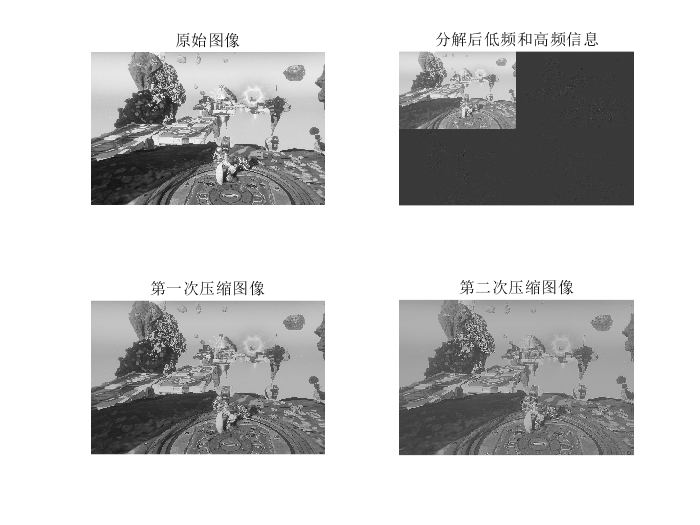
\includegraphics[width=0.9\textwidth]{untitled.png}
				\vspace{8cm} % 预留一些垂直空间
		}}
		\caption{实验结果图：(221)原始图像, (222)一级分解, (223)一级压缩, (224)二级压缩。}
		\label{untitled.png}
	\end{figure}
	% --- 占位符结束 ---
	
	实验共生成一个包含四个子图的图窗：
	\begin{itemize}
		\item \textbf{子图 (221) - 原始图像：} 显示了转换后的原始灰度图像，作为对比基准。
		\item \textbf{子图 (222) - 分解后低频和高频信息：}
		\begin{itemize}
			\item 左上角 (a1)：第 1 级低频重构，是原始图像的模糊缩小版。
			\item 右上角 (h1)：第 1 级水平高频重构，清晰地显示了图像中的垂直边缘。
			\item 左下角 (v1)：第 1 级垂直高频重构，清晰地显示了图像中的水平边缘。
			\item 右下角 (d1)：第 1 级对角高频重构，显示了对角线方向的细节。
		\end{itemize}
		\item \textbf{子图 (223) - 第一次压缩图像：} 显示了第 1 级的低频近似系数 \texttt{cal}。该图像在视觉上是原始图像的缩小版，保留了主要结构，但丢失了大量细节。这模拟了 4:1 的压缩效果（仅保留 LL1）。
		\item \textbf{子图 (224) - 第二次压缩图像：} 显示了第 2 级的低频近似系数 \texttt{ca2}。该图像比 \texttt{cal} 更加模糊和缩小，仅保留了最核心的轮廓信息。这模拟了 16:1 的压缩效果（仅保留 LL2）。
	\end{itemize}
	
	\subsection{结果分析}
	\begin{enumerate}
		\item \textbf{能量集中性验证：} 对比子图 (222) 中的四个分量，可以清晰地看到，图像的绝大部分视觉信息（能量）都集中在左上角的低频分量 \texttt{a1} 中，而三个高频分量 \texttt{h1}, \texttt{v1}, \texttt{d1} 只包含了边缘和纹理信息，且大部分区域接近于黑色（即系数接近 0）。这完美验证了小波变换的能量集中特性。
		\item \textbf{多级分解与压缩：} 对比子图 (223) 和 (224) 可以发现：
		\begin{itemize}
			\item 第 1 级近似 \texttt{cal} 保留了较多的图像信息，压缩比较低（4:1）。
			\item 第 2 级近似 \texttt{ca2} 丢失了更多细节，图像更模糊，但它占用的数据量更小（仅为原始图像的 1/16），实现了更高的压缩比。
			\item 这表明，在小波压缩中，分解的\textbf{层数}是一个关键参数。层数越多，低频分量（LLn）越小，压缩比越高，但图像质量损失也越大。
		\end{itemize}
		\item \textbf{代码分析：} 实验代码通过 \texttt{appcoef2} 仅提取低频分量来演示压缩思想。一个完整的压缩系统还应包括：
		\begin{itemize}
			\item 对高频系数 \texttt{ch1}, \texttt{cv1}, \texttt{cd1} 以及更高层的高频系数（\texttt{ch2}, \texttt{cv2}, \texttt{cd2}...）进行\textbf{阈值处理和量化}。
			\item 对量化后的所有系数（低频和高频）进行\textbf{熵编码}（如游程编码、霍夫曼编码）。
			\item 解压缩时，需要执行\textbf{熵解码}、\textbf{反量化}，并使用 \texttt{waverec2} 函数从所有系数 \texttt{c} 和结构 \texttt{s} 中\textbf{完全重构}图像。
		\end{itemize}
	\end{enumerate}
	
	\section{实验结论与心得}
	\subsection*{结论} % 使用无编号的 subsection
	\begin{enumerate}
		\item 小波变换能有效地将图像分离为低频（近似）和高频（细节）分量。
		\item 图像的主要能量集中在低频分量中，高频分量系数稀疏。
		\item 通过仅保留低频分量或对高频分量进行大量化，可以实现高效的有损图像压缩。
		\item 分解的层数越高，压缩比越高，但图像的保真度越低。
	\end{enumerate}
	
	\subsection*{心得体会} % 使用无编号的 subsection
	本次实验让我对小波变换的“时-频”局部化特性有了更深刻的理解。与傅里叶变换的“全局”性不同，小波能精确地捕捉到图像的局部特征（如边缘），并将其分离到高频子带。这正是它在图像压缩和去噪领域效果卓越的原因。
	
	实验中仅演示了压缩的核心原理，在后续学习中，我将尝试实现一个包含量化和重构的完整压缩/解压缩流程，并引入 PSNR（峰值信噪比）和 CR（压缩比）等客观指标来定量评估压缩性能。
	
	\section*{实验参考内容} % 无编号章节
	\begin{itemize}
		\item \textbf{参考文献：} \url{https://blog.csdn.net/chenyusiyuan/article/details/1881231?utm_source=blogxgwz0}
		\item \url{https://blog.csdn.net/xiaojidan2011/article/details/8099380}
	\end{itemize}
	
	% --- 附录 ---
	\appendix
	\section{实验代码}
	\begin{lstlisting}[language=Matlab, caption={MATLAB 实验代码}, label={lst:matlabcode}]
		clc;
		clear all;
		close all; % 清理工作空间
		clear; 
		X=imread('C:\Users\32610\Pictures\Screenshots\屏幕截图 2024-01-12 200049.png'); 
		X=rgb2gray(X);
		subplot(221); imshow(X); 
		title('原始图像'); 
		%对图像用小波进行层小波分解
		[c,s]=wavedec2(X,2,'bior3.7');
		%提取小波分解结构中的一层的低频系数和高频系数
		cal=appcoef2(c,s,'bior3.7',1);
		ch1=detcoef2('h',c,s,1); %水平方向
		cv1=detcoef2('v',c,s,1); %垂直方向
		cd1=detcoef2('d',c,s,1); %斜线方向
		%各频率成份重构
		a1=wrcoef2('a',c,s,'bior3.7',1);
		h1=wrcoef2('h',c,s,'bior3.7',1);
		v1=wrcoef2('v',c,s,'bior3.7',1);
		d1=wrcoef2('d',c,s,'bior3.7',1);
		c1=[a1,h1;v1,d1];
		subplot(222),imshow(c1,[]);
		title ('分解后低频和高频信息');
		%进行图像压缩
		%保留小波分解第一层低频信息
		%首先对第一层信息进行量化编码
		ca1=appcoef2(c,s,'bior3.7',1);
		ca1=wcodemat(ca1,440,'mat',0);
		%改变图像高度并显示
		ca1=0.5*ca1;
		subplot(223);imshow(cal,[]);
		title('第一次压缩图像');
		%保留小波分解第二层低频信息进行压缩
		ca2=appcoef2(c,s,'bior3.7',2);
		%首先对第二层信息进行量化编码
		ca2=wcodemat(ca2,440,'mat',0);
		%改变图像高度并显示
		ca2=0.25*ca2;
		subplot(224);imshow(ca2,[]);
		title('第二次压缩图像');
	\end{lstlisting}
	
\end{document}
% --- 文档结束 ---